\documentclass[11pt, a4paper]{article}
\usepackage[margin=1in]{geometry}

\usepackage{lmodern}
\fontfamily{lmdh}\selectfont

\usepackage{graphicx}
\graphicspath{{../}}

\usepackage{titlesec}
\titleformat*{\section}{\large\bfseries}

\usepackage{caption}

\usepackage{subcaption}

\usepackage[style=authoryear-ibid,backend=biber]{biblatex}
\renewcommand*{\nameyeardelim}{\addcomma\space}
\addbibresource{ag_bib.bib}

\usepackage{verbatim}

\usepackage[section]{placeins}

\title{\Large\bfseries SMART Analysis for Roadwork Prioritisation}
\author{\large Amanjit Gill}
\date{\small \today}

\begin{document}
    
    \maketitle

    \section{Abstract}

    The Victorian government is engaged in an extensive program of public infrastructure works, with a specific focus on road and rail \parencite{a1}. However, the process by which the government identifies, prioritises and commits to these projects is not publicly documented, and this has led to some doubt as to whether roadworks funding is being targeted in the most beneficial way. 

    This analysis makes the case for wider adoption of MCDM (multi-criteria decision making) methods in planning processes, and demonstrates the use of one such method, SMART, in the identification of a road location that is most in need of safety improvements. This procedure is shown to be effective and robust for such purposes, and an entreaty is made to the Victorian government to employ MCDM in a program of transparent and defensible decision making.

    \section{Introduction}

    The purpose of this analysis is to assess and shortlist the most dangerous road locations in Victoria, and then to use a multi-criteria decision analytics approach to select the location that is most in need of major redevelopment.

    The impetus for this undertaking came from an observation that was recently made in the author's locality in Victoria. This observation was of a local road and intersection that have undergone a costly, time-consuming and disruptive reconstruction process \parencite{a2}, only to appear, at the conclusion of these works, to have changed very little in terms of both function and appearance.

    The road and intersection in question have never been marked by severe traffic congestion or frequent collisions. Publicly available data show that the intersection, denoted in records by the identifier 332806, was involved in only 4 collisions in the five-year period to June 2020 \parencite{a3}. Furthermore, the government has not published - or validated - the process by which this location was prioritised.

    By contrast, the method proposed in the present analysis, multi-criteria decision-making (MCDM), has been validated as an approach to road infrastructure planning by researchers. The analytical heirarchy process (AHP) has been used to assess and prioritise road surface repairs \parencite{a4}, and a hybrid approach combining multi-criteria and cost-benefit analyses has also been done \parencite{a5}. In addition, Patel et al. (2017) validates the applicability of SMART (simple multi-attribute rating technique) across a broad range of technical and planning activities.

    The present analysis is, however, limited in that an exhaustive investigation and primary data collection cannot be done due to time and budget constraints. Because of this, care has been taken to only select attributes about which information is already available, while ensuring that the main causes of road risk are adequately covered. To this end, the author has made use of data published online by government bodies, either as downloadable data files or as interactive web applications.

    Despite these limitations, a considerable amount of relevant data have been found, leading to the shortlisting and subsequent selection of a road location that is most in need of redevelopment. Furthermore, the process has been found to be robust against changes. It is hoped that this analysis can provide a blueprint from which the Victorian government may make sound, evidence-based, planning decisions.

    \section{Problem Identification}

    The identification of road improvement as a suitable subject for a decision analytics problem came about as a result of the author's failure to locate information justifying the major reconstruction works being undertaken at the intersection mentioned earlier. 

    Attempts were made to establish the rationale for the Victorian government's decision to redevelop this road and intersection. These attempts have been fruitless; the only available information pertains to the purported benefits of the project, and a discussion of some community consultation that occurred after a commitment was already made to proceed \parencite{a7}. 

    This was followed by an examination of Victorian government websites, in order to find the following:

    \begin{itemize}
        \item a list of "black spot" intersections; these are intersections that are marked as particularly dangerous, which are sometimes allocated funding for improvement works by the federal government \parencite{a8}
        \item any form of analysis or documentation, such as a cost-benefit analysis or a business case, that explains how and why any road project has been approved in recent years
    \end{itemize}

    While they may be publicly available, none of these documents could be found within a reasonable amount of time. There is documentation on the processes that VicRoads, the body responsible for smaller projects like the installation of safety barriers, uses when identifying and prioritising potential targets for improvement \parencite{a9}. However, it is not apparent that this has been used in major construction projects, which are outside VicRoads' scope of work.

    From the above, it is apparent that the government does provide information about the benefits of major improvement works, but only after it has committed the resources. Additionally, while there is some information - through VicRoads - about the processes the government might use, there is no publicly available evidence of their use in specific projects.
    
    It is this absence of evidence of a methodical approach to roadwork prioritisation that motivates the present analysis. MCDM has already been endorsed for its utility in transport planning projects. Of particular note is the encouragement of MCDM methods by Infrastructure Australia and the Queensland Department of Transport and Main Roads \parencite{a10}, both of which have published detailed technical guidelines on assessing projects. In addition, research such as that by Akpan and Morimoto (2021), wherein multi-criteria methods are used to prioritise repairs to a large number of rural roads, as well as the studies mentioned earlier, comprehensively build the case for Victorian adoption of MCDM in road infrastructure planning.
    
    However, the aforementioned studies involve extensive data collection and the use of specialised equipment to quantify the specified attributes; by contrast, the author of the present study seeks to show that a desktop analysis, relying only on data that are already available, can be a capable and efficient stand-in when resources are constrained.
    
    \section{Solution Approach}

    SMART (simple multi-attribute rating technique) has been deemed the most appropriate method for evaluating different road locations for redevelopment. This procedure provides a methodical approach that gives proportionate consideration to competing objectives, preventing a decision that overemphasises one objective to the detriment of others \parencite{a13}. In addition, the attention paid to the selection and measurement of attributes enables a decision-making process that is transparent and defensible \parencite{a13}, qualities that are particularly important for government accountability.

    The SMART approach is, as its name suggests, simple. As outlined by Patel et al. (2017), the procedure involves the following actions:

    \begin{enumerate}
        \item Identify the person(s) who will make the decision.
        \item  Identify the problem.
        \item  Identify the decision alternatives that should be considered.
        \item  Select attributes (criteria) upon which to compare the alternatives.
        \item  Order the attributes from most important to least.
        \item  Assign each attribute a weight that represents its importance, relative to the other attributes.
        \item  Normalise the attribute weights.
        \item  For each attribute, rank the alternatives such that a rank represents the degree to which the \item  decision maker prefers this alternative to the others.
        \item  For each alternative, compute a weighted sum using its own scores and the attribute weights.
        \item  Make a decision - this is likely to be the alternative with the highest weighted sum.
    \end{enumerate}

    At the end of this procedure, the alternative with the highest weighted sum is considered to be the strongest candidate when the competing criteria are considered together, with proportionate consideration given to each one.

    AHP (analytical heirarchy process) was also considered, but this is more appropriate when many of the selected attributes are non-quantifiable. In the present case, all of the selected attributes are quantifiable, either directly or indirectly, making them good candidates for evaluation through value functions such as those used in SMART.

    In addition, risk-based models like decision trees are also not appropriate, because the problem at hand is not one of probabilities and risks (the outcome of improving a dangerous road or intersection is almost certainly an increase in safety and a decrease in collisions); what is being contested is which location represents the most beneficial use of resources.

    \section{Results and Discussion}

    \subsection{Shortlisting of Alternatives}

    As aforementioned, once the decision maker (in this case, the author of the present analysis) and the problem (choosing a road location to upgrade) has been identified, the decision alternatives must be determined. There are 150,000 km of road available to general traffic in Victoria \parencite{a14}; therefore, in order to identify the locations most in need of redevelopment, road accident statistics were obtained from VicRoads \parencite{a3}. The six locations with the most accidents over the reporting period were chosen as decision alternatives (refer to Table \ref{t4}).

    \begin{table}[!ht]
        \centering
        \begin{tabular}{|l|l|l|l|l|l|l|l|l|l|}
        \hline
            ~ & Node ID & Latitude & Longitude & Address    & Suburb   \\ \hline
            A & 36335 & -37.7923 & 144.9684 & cnr Lygon St, Princes St    & Carlton Nth   \\ \hline
            B & 10592 & -37.9332 & 145.1568 & cnr Springvale Rd, Police Rd, Princes Hwy    & Springvale   \\ \hline
            C & 42680 & -37.9612 & 145.3612 & cnr Wellington Rd, Berwick Rd    & Belgrave Sth   \\ \hline
            D & 45524 & -37.8050 & 144.6959 & cnr Boundary Rd, Derrimut Rd    & Derrimut   \\ \hline
            E & 29361 & -37.7849 & 144.9751 & cnr Canning St, Richardson St    & Carlton Nth   \\ \hline
            F & 35605 & -37.9822 & 145.0714 & cnr Nepean Hwy, Warrigal Rd    & Mentone   \\ \hline
        \end{tabular}
        \caption{Shortlisted Locations}
        \label{t4}
    \end{table}

    \subsection{Selection of Attributes}

    The following attributes were chosen because they are easily measurable or quantifiable; and, when taken together, they form a sufficiently broad and complete picture of the importance and urgency of a potential road development project.

    \hfill \break
    Danger:
    \begin{itemize}
        \item This is decomposed into two quantifiable sub-attributes, Severe Accidents and Other Accidents.
        \item The figures for these sub-attributes are obtained from the VicRoads statistics aforementioned \parencite{a3}, and are considered a suitable indicator of danger level.
        \item A third sub-attribute, Fatal Accidents, has been removed, because there were too few fatal accidents at the shortlisted locations to impact the analysis. 
    \end{itemize}

    \hfill \break
    Congestion:
    \begin{itemize}
        \item This encapsulates the high traffic volumes that often characterise hazardous driving conditions. According to one insurance company, 27\% of its collision claims are for accidents that occurred between 8-9am and 3-6pm on weekdays \parencite{a15}.
        \item VicRoads has published traffic volume data \parencite{a16}, but this is available only as a very large file that is unable to be processed by the author's data analysis equipment. Therefore, the extent of congestion at a location has been estimated with a "congestion ratio"; this is a ratio of the time it takes to travel through a 1km section, at peak and off-peak times. These travel times are obtained from a web application \parencite{a17}.
    \end{itemize}

    \hfill \break
    Benefaction:
    \begin{itemize}
        \item This attribute seeks to capture the extent to which the local community would benefit from a road location being redeveloped, and has been decomposed into two more easily quantifiable sub-attributes, Proximity to Vulnerable Populations and Size of Local Population.
        \item The closer a road location is to schools, hospitals and aged care facilities, the more there is to be gained from making that location safer. Therefore, in this analysis, locations that are very close to these facilities are preferred. Each location is given a weighted sum of its distance from the three categories of facility. The distances have been acquired from a web application \parencite{a17}.
        \item When a road is improved, all of the residents local to that area are potentially beneficiaries of this improvement, as they are likely to use that road. While it is difficult to estimate the number of people living directly in the vicinity of a location, it is easy to obtain data on the population of a local government area \parencite{a18}. Therefore, in this analysis, a location within a high-population municipality is preferred.
    \end{itemize}

    Together, these attributes are considered to contribute to the relative "exigency" of a road development project; that is, a blend of the importance and urgency of making a location safer. As shown in Figure \ref{f3}, "costs" and "benefits" are not being measured in this analysis; rather, it is exigency that is being measured, which this is an entity that has no cost.

    \begin{figure}[hbt!]
        \centering
        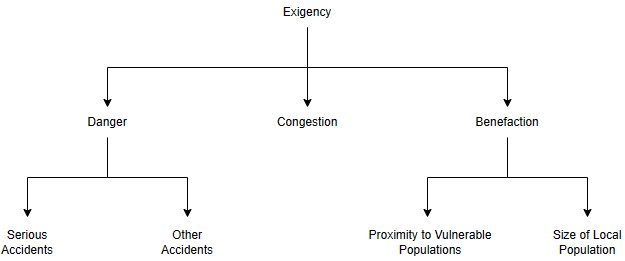
\includegraphics[width=\textwidth]{figures/3.jpg}
        \caption{Value Tree}
        \label{f3}
    \end{figure}

    Tables \ref{t5}-\ref{t8} contain the raw data that have been collected for the six alternatives.

    \begin{table}[!ht]
        \centering
        \begin{tabular}{|l|l|l|l|l|l|l|l|l|l|}
        \hline
            ~ & Total & Fatal & Serious & Other       \\ \hline
            A & 25 & 0 & 10 & 15       \\ \hline
            B & 23 & 0 & 14 & 9       \\ \hline
            C & 23 & 1 & 9 & 13       \\ \hline
            D & 22 & 0 & 8 & 14       \\ \hline
            E & 21 & 0 & 7 & 14       \\ \hline
            F & 21 & 0 & 9 & 12       \\ \hline
        \end{tabular}
        \caption{Road Accidents}
        \label{t5}
    \end{table}

    \begin{table}[!ht]
        \centering
        \begin{tabular}{|l|l|l|l|l|l|l|l|l|l|}
        \hline
            ~ & School & Hospital & Aged Care        \\ \hline
            A & 0.6 & 1.9 & 0.5        \\ \hline
            B & 0.24 & 3.9 & 0.21        \\ \hline
            C & 2.8 & 12.9 & 10        \\ \hline
            D & 3.2 & 6.6 & 3.9        \\ \hline
            E & 1 & 1.5 & 0.6        \\ \hline
            F & 0.16 & 2.8 & 0.45        \\ \hline
        \end{tabular}
        \caption{Proximity to Vulnerable Populations}
        \label{t6}
    \end{table}

    \begin{table}[!ht]
        \centering
        \begin{tabular}{|l|l|l|l|l|l|l|l|l|l|}
        \hline
            ~ & 2:00 AM & 5:00 PM & Congestion Factor        \\ \hline
            A & 2 & 9 & 4.5        \\ \hline
            B & 2 & 3 & 1.5        \\ \hline
            C & 1 & 1 & 1.0        \\ \hline
            D & 2 & 3 & 1.5        \\ \hline
            E & 3 & 4 & 1.3        \\ \hline
            F & 2 & 3 & 1.5        \\ \hline
        \end{tabular}
        \caption{Congestion}
        \label{t7}
    \end{table}

    \begin{table}[!ht]
        \centering
        \begin{tabular}{|l|l|l|}
        \hline
            ~ & LGA & Population (1000s)  \\ \hline
            A & borders Yarra and Melbourne & 287  \\ \hline
            B & borders Monash and Greater Dandenong & 373  \\ \hline
            C & Yarra Ranges & 160  \\ \hline
            D & borders Wyndham and Melton & 456  \\ \hline
            E & Yarra & 103  \\ \hline
            F & Kingston & 167  \\ \hline
        \end{tabular}
        \caption{Local Population}
        \label{t8}
    \end{table}

    \subsection{Weighting of Attributes and Alternatives}

    All of the attributes are quantifiable; therefore, a different value function has been used to scale each one (refer to Appendix B). These functions are subjective in that they are based on the author's own judgements. They are created with the "bisection" method that has been described in Goodwin (2014); in this analysis, they mostly appear to be nearly linear, not following the idealised curved examples shown in the text mentioned. However, linear value functions are considered acceptable \parencite{a6}.

    The relative weight of each attribute has also been assessed and normalised (refer to Table \ref{t9}); again, subjective judgements by the author have been used.

    \begin{table}[!ht]
        \centering
        \begin{tabular}{|l|l|l|l|l|l|l|l|}
        \hline
            ~ & Raw Weight & Norm. Weight       \\ \hline
            Serious Accidents & 100 & 27       \\ \hline
            Other Accidents & 80 & 22       \\ \hline
            Congestion & 80 & 22       \\ \hline
            Proximity to Vulnerable Populations & 60 & 16       \\ \hline
            Local Population & 50 & 14       \\ \hline
            Sum of Weights & 370 & 100       \\ \hline
        \end{tabular}
        \caption{Normalised Weights}
        \label{t9}
    \end{table}

    \subsection{Evaluation of Alternatives}

    Each location alternative has been scored on all attributes, using the value functions. Then a weighted sum of these scores has been calculated using the attribute weights. These final evaluations can be found in Table \ref{t10}. Based on this analysis, it is clear that location A has the most pressing need for improvement works.

    \begin{table}[!ht]
        \centering
        \begin{tabular}{|l|l|l|l|l|l|l|l|}
        \hline
            ~ & Serious Accidents & Other Accidents & Congestion & Proximity & Population & Weighted Sum   \\ \hline
            A & 50 & 100 & 100 & 100 & 72 & 82.7   \\ \hline
            B & 100 & 0 & 25 & 95 & 87 & 59.6   \\ \hline
            C & 33 & 67 & 0 & 0 & 29 & 27.3   \\ \hline
            D & 17 & 83 & 25 & 35 & 100 & 47.1   \\ \hline
            E & 0 & 83 & 22 & 98 & 0 & 38.6   \\ \hline
            F & 33 & 50 & 25 & 100 & 33 & 45.8   \\ \hline
        \end{tabular}
        \caption{Weighted Sum}
        \label{t10}
    \end{table}

    Unlike other SMART analyses, there is no cost attribute to model, and therefore no efficient frontier; the prevailing alternative is simply the one with the most exigency.

    \subsection{Sensitivity Analysis}

    In order to assess the robustness of this model, three sensitivity analyses were carried out, with the following considerations in mind:

    \begin{enumerate}
        \item Serious Accidents has the highest weight of all the attributes. Changes to this weight may have significant impacts on the final decision; this possibility needs to be either confirmed or ruled out.
        \item Although this is counter to the principles of public service, important government decisions - even those involving health and safety - are sometimes made for political advantage \parencite{a19}. A government might determine that focusing on locations with high congestion and high local populations will deliver improvements that are more noticeable to more people, thereby increasing the government's chances of re-election. Therefore, it would be useful to ascertain whether this model is sensitive to changes in the weights of those two attributes.
    \end{enumerate}

    Graphs for these sensitivity analyses can be found in Appendix C. It is clear that if the weights of any of the three attributes of interest (Serious Accidents, Congestion and Local Population) are altered in any way, then location A will remain the preferred alternative, regardless of how low or high the altered attribute is weighted. This seems remarkable, but is not surprising when one considers that location A scored 100 on three out of five attributes, making it very difficult to dislodge as the preferred redevelopment location. 

    The sensitivity analyses also show that location C will always be the least-preferred alternative, regardless of how the three attributes of interest are weighted. Again, this is not entirely surprising, because this area is located on the outskirts of Melbourne, so it scored 0 on Congestion and Proximity to Vulnerable Populations, and relatively low on Local Population.

    \subsection{Appraisal of the approach}

    The stability of the analysis outcome confirms that for this problem, the decisions to use SMART over other methods, as well as to define the problem in terms of exigency rather than traditional costs and benefits, has resulted in a robust tool that can successfully be applied to road infrastructure planning activities.

    \section{Conclusion}

    This analysis used SMART, a multi-criteria decision making method, to select a road location that is most in need of improvement in terms of traffic safety. The successful application of this approach, and its robustness against changes, validates its use in the Victorian context.

    There are, however, limitations to consider. The available data on traffic volumes was unusable, and the "congestion ratio", which is based upon online estimates of travel time, is a crude replacement. Ideally, if this analysis were to be repeated, real traffic data would be acquired.
    
    Nevertheless, it is hoped that this analysis provides a blueprint for how the Victorian government can adopt a more methodical, transparent and defensible approach to project planning.

    \newpage
    \printbibliography

    \newpage
    \section*{Appendix A: Sensitivity Analysis for Task 2}

        \begin{figure}[!ht]
            \centering
            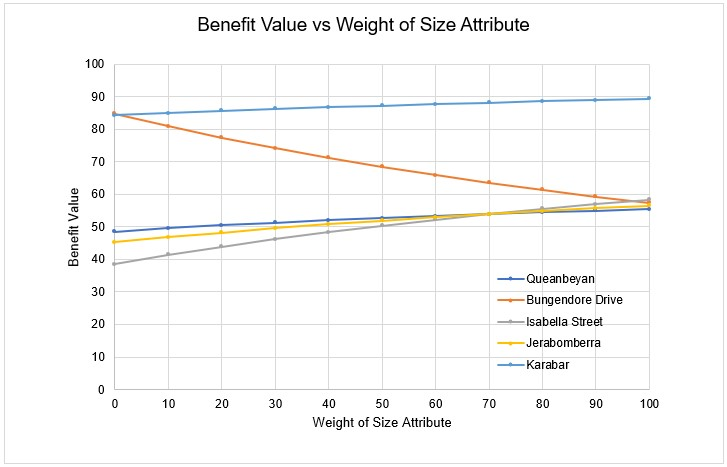
\includegraphics[width=\textwidth]{appendices/1a.jpg}
        \end{figure}

        \begin{figure}[!ht]
            \centering
            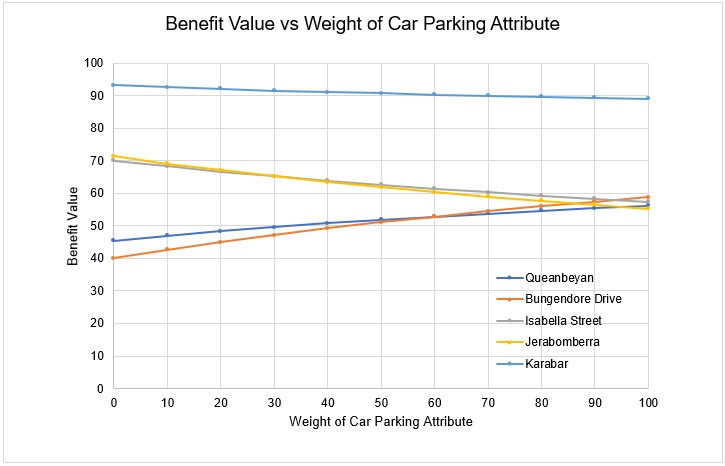
\includegraphics[width=\textwidth]{appendices/1b.jpg}
        \end{figure}

        \begin{figure}[!ht]
            \centering
            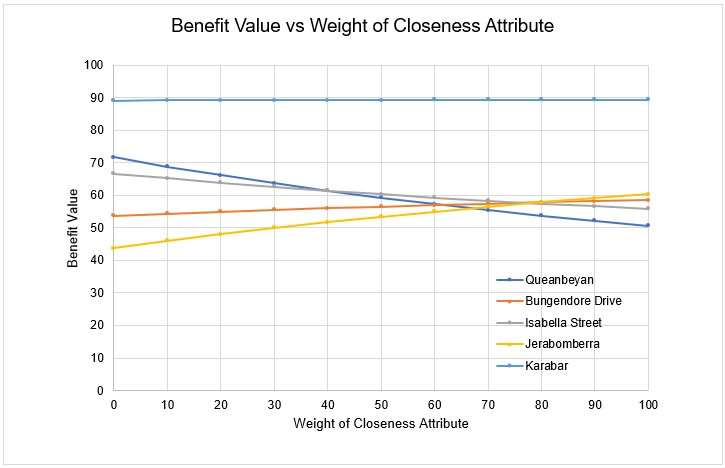
\includegraphics[width=\textwidth]{appendices/1c.jpg}
        \end{figure}

    \newpage
    \section*{Appendix B: Value Functions For Task 3}

        \begin{figure}[!ht]
            \centering
            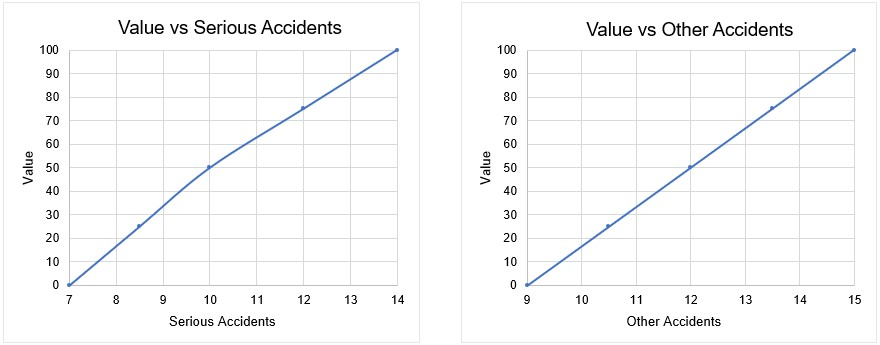
\includegraphics[width=\textwidth]{appendices/2a.jpg}
        \end{figure}

        \begin{figure}[!ht]
            \centering
            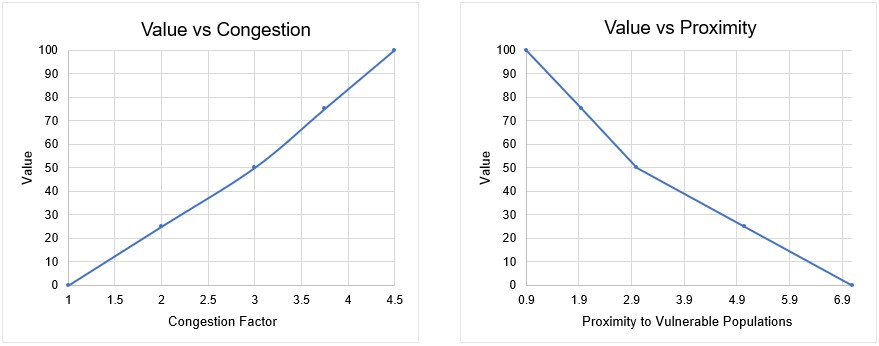
\includegraphics[width=\textwidth]{appendices/2b.jpg}
        \end{figure}

        \begin{figure}[!ht]
            \centering
            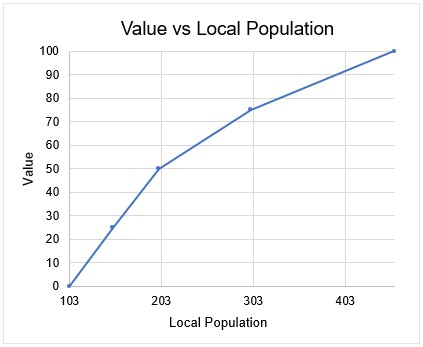
\includegraphics[width=\textwidth]{appendices/2c.jpg}
        \end{figure}

    \newpage
    \section*{Appendix C: Sensitivity Analysis For Task 3}

        \begin{figure}[!ht]
            \centering
            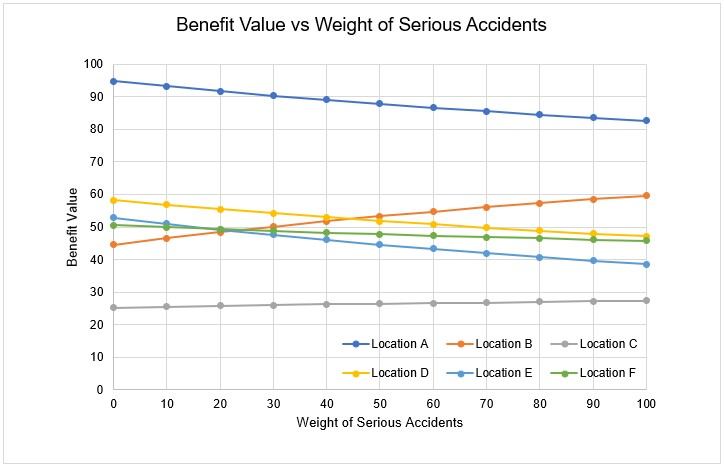
\includegraphics[width=\textwidth]{appendices/3a.jpg}
        \end{figure}

        \begin{figure}[!ht]
            \centering
            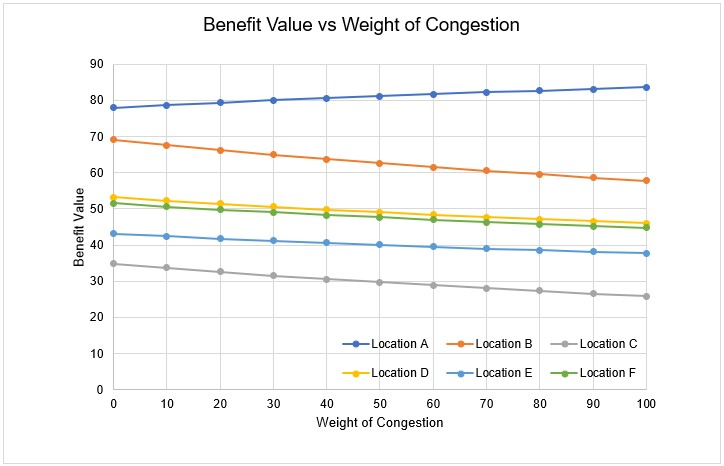
\includegraphics[width=\textwidth]{appendices/3b.jpg}
        \end{figure}

        \begin{figure}[!ht]
            \centering
            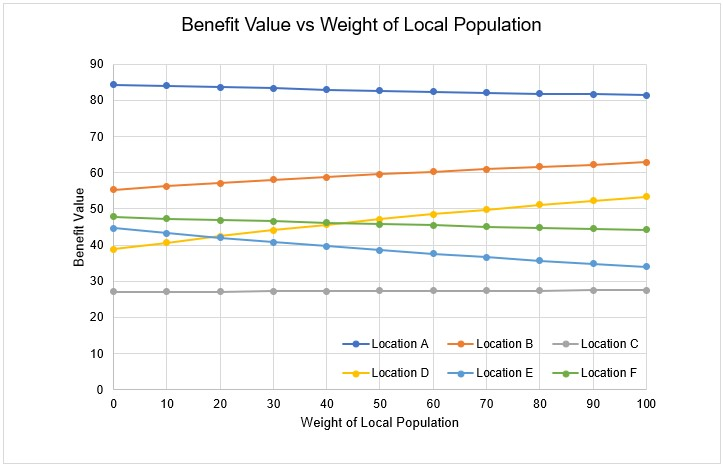
\includegraphics[width=\textwidth]{appendices/3c.jpg}
        \end{figure}

\end{document}

